\documentclass{article}
\usepackage[final]{neurips}
\usepackage[framemethod=tikz]{mdframed}
\usepackage{lipsum,amsthm,amssymb}
\definecolor{mycolor}{rgb}{0.122, 0.435, 0.698}
\newmdenv[innerlinewidth=0.5pt, roundcorner=4pt,linecolor=mycolor,innerleftmargin=6pt,
innerrightmargin=6pt,innertopmargin=6pt,innerbottommargin=6pt]{mybox}
\usepackage[utf8]{inputenc} % allow utf-8 input
\usepackage[T1]{fontenc}    % use 8-bit T1 fonts
\usepackage{hyperref}       % hyperlinks
\usepackage{url}            % simple URL typesetting
\usepackage{booktabs}       % professional-quality tables
\usepackage{amsfonts}       % blackboard math symbols
\usepackage{nicefrac,tcolorbox}       % compact symbols for 1/2, etc.
\usepackage{amsmath}
\usepackage{enumitem}
\usepackage{microtype}      % microtypography
\usepackage{graphicx,caption}
\usepackage{xepersian}
\settextfont{XB Niloofar}
\setdigitfont{XB Niloofar}
\raggedbottom
\usepackage[labelformat=empty]{caption} 

\title{
	\vspace{-0.8em}
تمرین سری ششم درس نظریه گروه‌ها - دکتر رضاخانی
\\
{\normalsize
\textbf{مهلت تحویل:
جمعه ۲۱ اردیبهشت ماه سال 1403 تا ساعت 59:23
\\
\vspace{-0.4em}
از طریق سامانه
\href{https://cw.sharif.edu/}{درس‌افزار شریف}
}
}
\vspace{-0.6em}
}
\usepackage[utf8]{inputenc}

\usepackage[english]{babel}
\setlength{\parindent}{3.5em}
\setlength{\parskip}{0.5em}
\renewcommand{\baselinestretch}{1.0}

\usepackage{calrsfs}
\DeclareMathAlphabet{\pazocal}{OMS}{zplm}{m}{n}
\newcommand{\La}{\mathcal{L}}
\newcommand{\Lb}{\pazocal{L}}

\newtcolorbox{boxes}[3][]
{
	colframe = #2!25,
	colback  = #2!10,
	coltitle = #2!40!black,  
	title    = {\textbf{#3}},
	#1,
}

\newenvironment{exercise}[3][\unskip]{%
	\par
	\noindent
	\textbf{تمرین
		#1
		[#2 امتیاز] 
		\def\temp{#3}\ifx\temp\empty
		: 
		\else
		: #3 \vspace{0.5em} \\ \noindent
		\fi
}}{}


\author{
حسین محمدی\\
  \lr{
  		\href{mailto:hossein.mohammadi.00427@gmail.com}{\texttt{	hossein.mohammadi.00427@gmail.com}}} \\
  \And
  زهرا کبیری\\
 \lr{
  		\href{mailto:kabiri.zahra98@gmail.com}{ \texttt{kabiri.zahra98@gmail.com}}}\\
  }

\begin{document}


\begin{minipage}{0.1\textwidth}% adapt widths of minipages to your needs
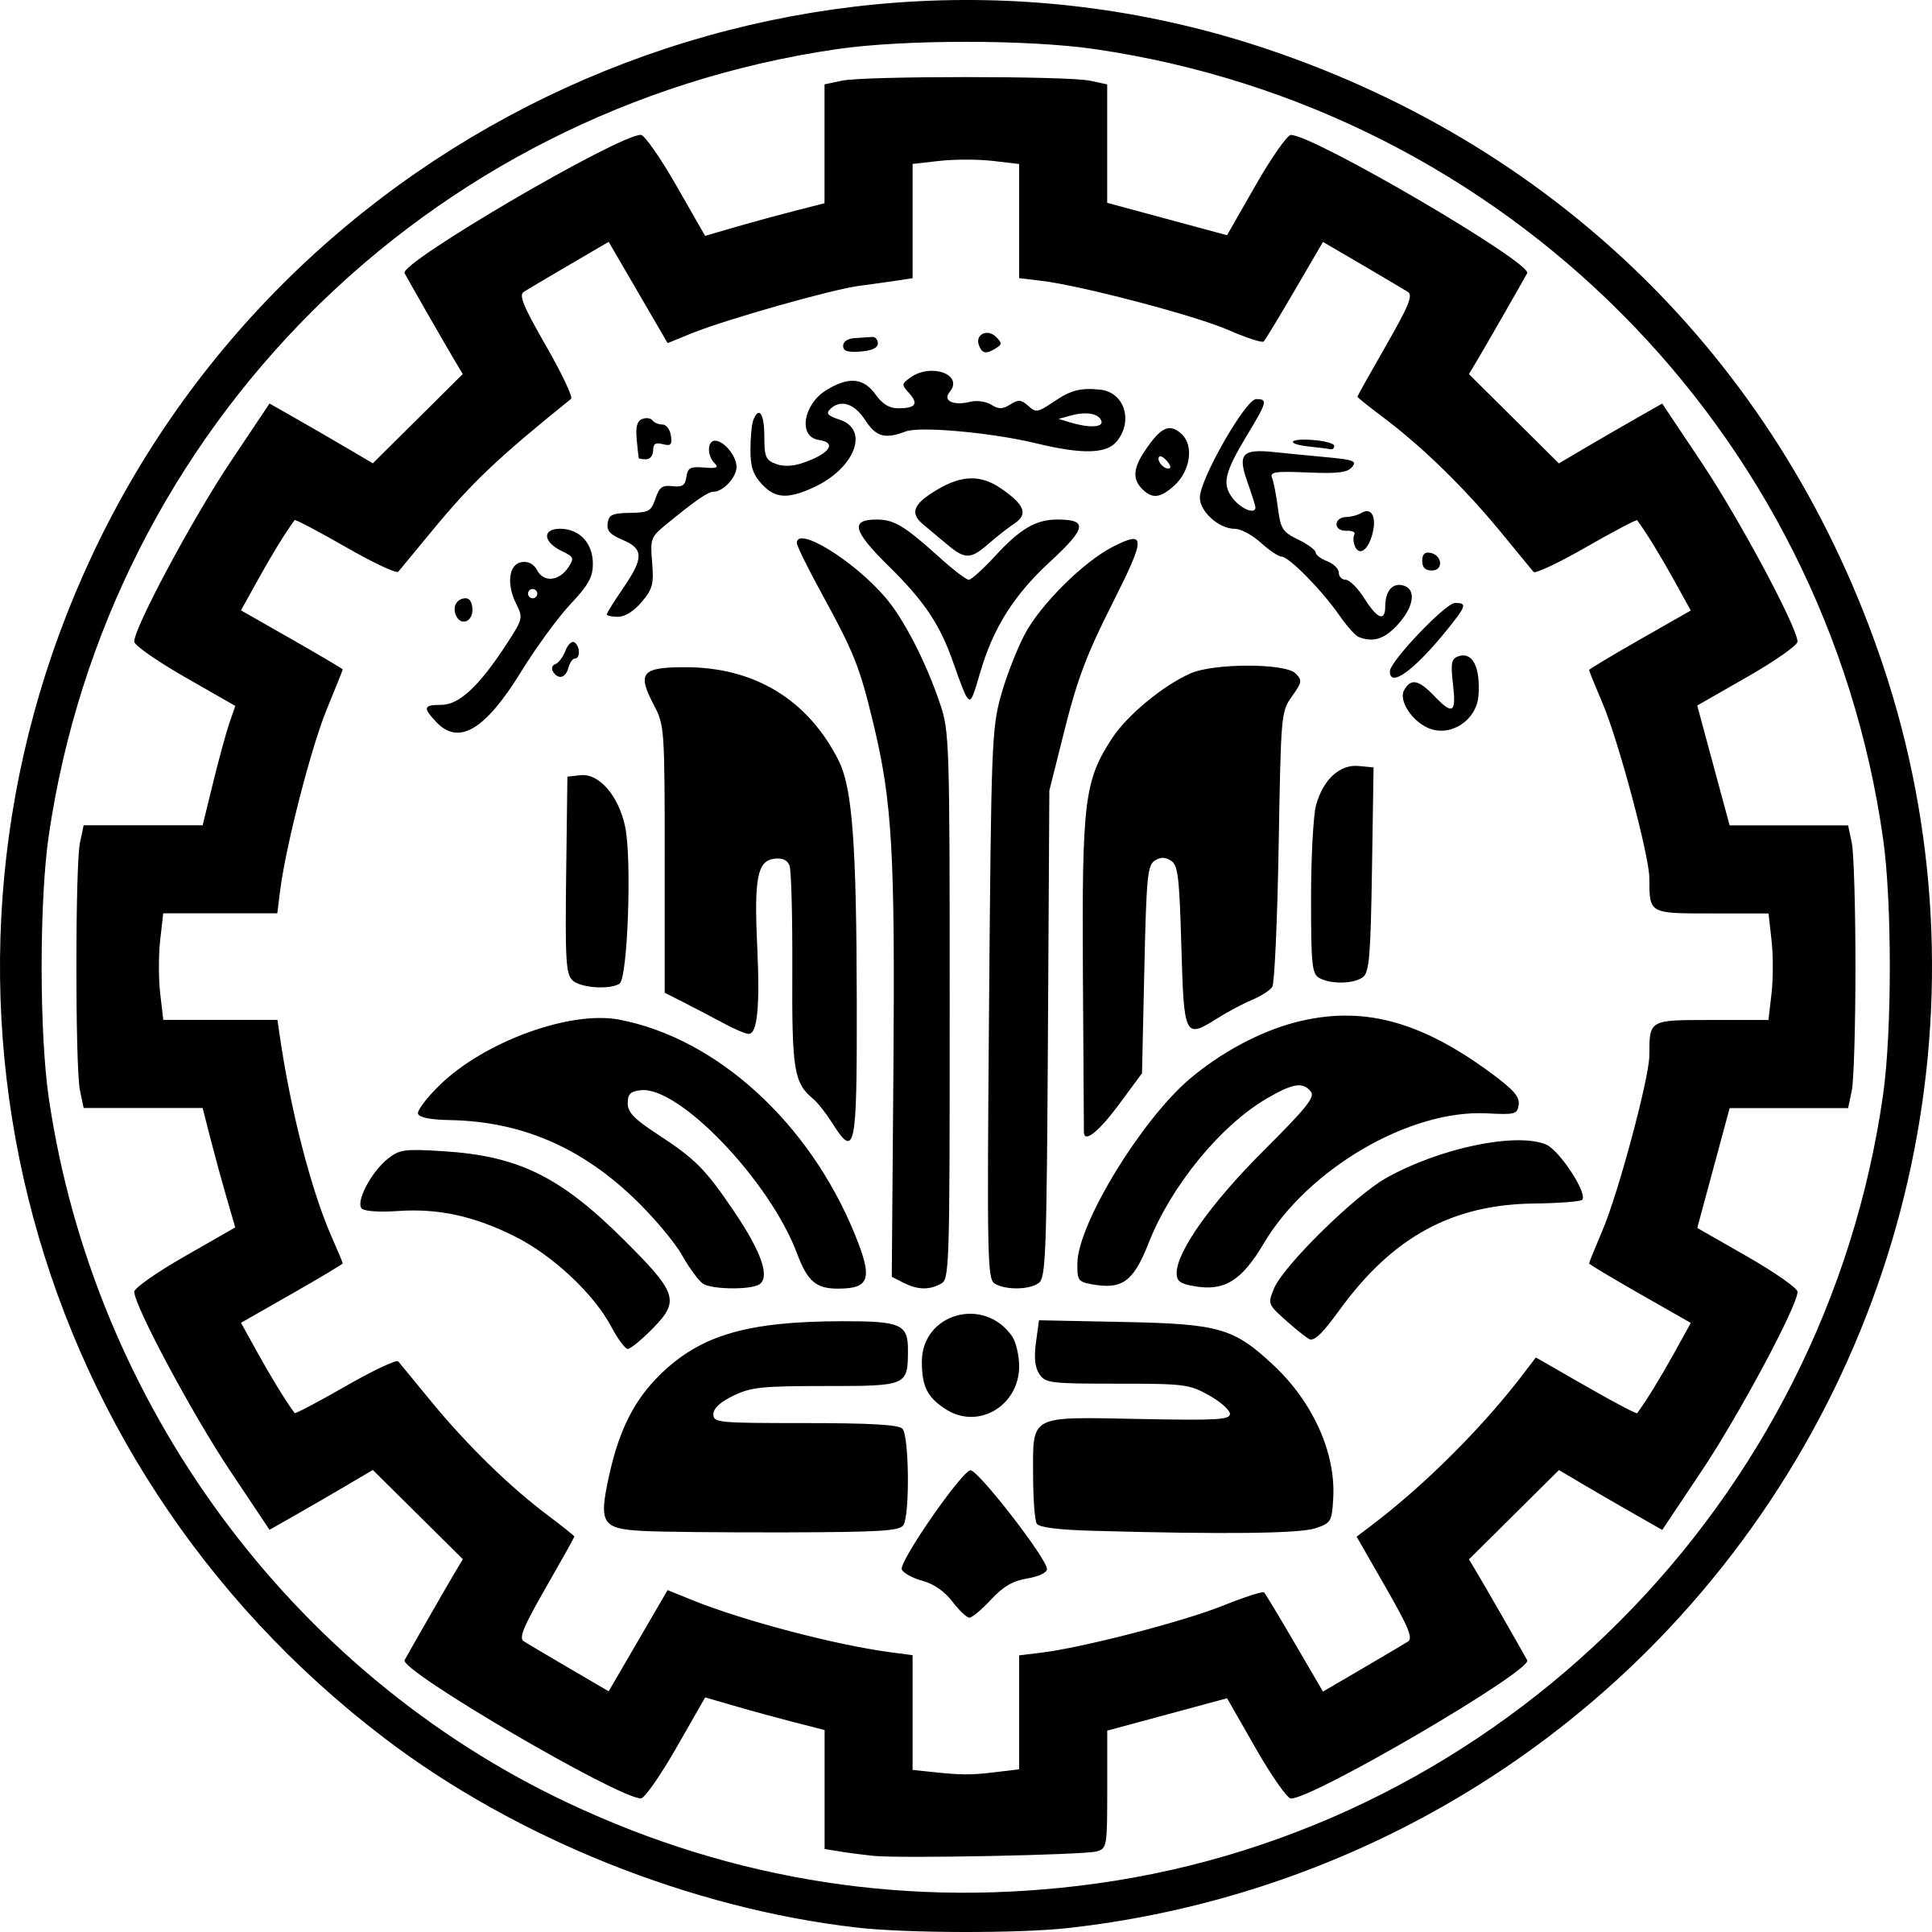
\includegraphics[width=1.1cm]{sharif-logo.png}
\end{minipage}%
\hfill%
\begin{minipage}{0.9\textwidth}\raggedleft
دانشگاه صنعتی شریف\\
زمستان ۱۴۰۲ - بهار ۱۴۰۳\\
\end{minipage}

\makepertitle


\begin{exercise}[۲۵]{40}{زمان و تکانه نظیر آن}
در حالت کلی که لاگرانژی بتواند تابع زمان باشد، کنش یک تئوری بر حسب لاگرانژی آن این‌طور نوشته می‌شود:
\begin{equation*}
    S=\int_{}^{} \mathcal{L} (t,q,\dot{q}) \,dt
\end{equation*}
می‌توانیم خود زمان را مانند یک مختصه بگیریم که همراه 
$q$ 
بعد از حل معادله حرکت، تابعی از یک پارامتر دیگر 
$\tau$ 
است. شکل زیر این را نشان می‌دهد. \\
\begin{center}
\begin{figure}[!h]
    \centering
    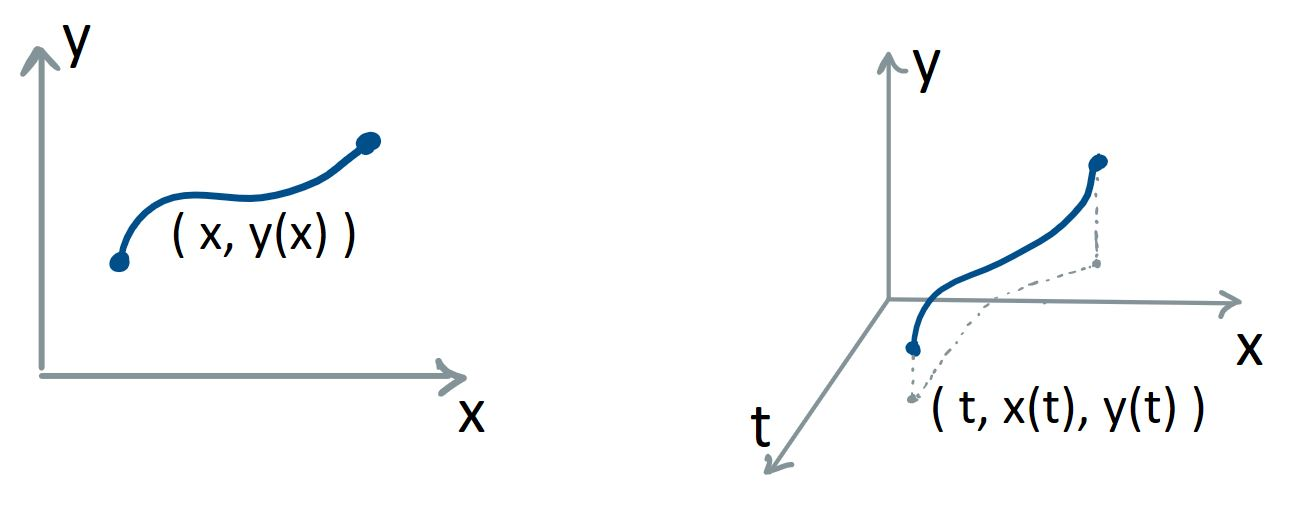
\includegraphics[width=0.6\textwidth]{Pics/fig1.JPG}
    \caption{
    شکل۱: 
شکل الف مسیر 
$(x,y(x))$ 
که جواب معادله حرکت است را نشان می‌دهد. هر مختصه تابعی از زمان است. 
$(x(t),y(t))$ 
می‌توان به زمان به عنوان پارامتر این خم در صفحه 
$(x,y)$ نگاه کرد.\\
شکل ب حالتی را که تئوری می‌تواند تابعی از زمان باشد نشان می‌دهد. مسیری که جواب معادله حرکت است را می‌توان بر اساس پارامتر این خم در فضای سه بعدی 
$(t,x,y)$ 
نشان داد. یعنی 
$(t(\tau),x(\tau),y(\tau))$
    }
\end{figure}
\end{center}


اگر نام این پارامتر را 
$\tau$ 
بگذاریم، جواب معادله حرکت به صورت 
$t(\tau)$ 
و 
$q(\tau)$ 
به دست می‌آید که: 
\begin{equation*}
    \dot{q}=\frac{dq}{dt}=\frac{d\tau}{dt}\frac{dq}{d\tau}=\frac{q'}{t'}
\end{equation*}
در اینجا مشتق‌های نسبت به 
$t$ 
و 
$\tau$ 
را چنین نمادگذاری کرده‌ام: 
$(\dot{f}:= \frac{df}{dt}, \quad f':=\frac{df}{d\tau})$
\\
الف) اگر همین کنش را برای پارامتر 
$\tau$ 
به عنوان زمان جدید بخواهیم به دست آوریم یعنی:
\begin{equation*}
    S=\int_{}^{} \mathcal{L} (t,q,\dot{q}) \,dt
    =\int_{}^{} \Tilde{\mathcal{L}} (t,q,,t',q') \,d\tau
\end{equation*}
تابع 
$\Tilde{\mathcal{L}}$ 
را پیدا کنید. 
\\
می‌توان گفت حالا خود 
$t$ 
همانند مختصه 
$q$ 
است و 
$\tau$ 
نقش زمان را بازی می‌‌کند. تئوری بازنویسی شده 
$\Tilde{\mathcal{L}}$ 
را بر حسب مختصات 
$q^{\alpha}=(t,q)$
نوشتیم که مشتق‌های آن نسبت به 
$\tau$ 
گرفته شده است
$\left((q^{\alpha})'=\frac{dq^{\alpha}}{d\tau}=(t',q')\right)$.
\\
ب) معادله اویلر-لاگرانژ را برای این لاگرانژی جدید 
$\Tilde{\mathcal{L}}$
نسبت به 
$\tau$ 
حل کنید یعنی:
\begin{equation*}
    \frac{\partial\Tilde{\mathcal{L}}}{\partial q^{\alpha}}-\frac{d}{d\tau} \frac{\partial\Tilde{\mathcal{L}}}{\partial (q^{\alpha})'}=0
\end{equation*}
آيا همان معادله حرکت مربوط به 
$\mathcal{L}$ 
را می‌دهد؟ 
$\left(    \frac{\partial\mathcal{L}}{\partial q}-\frac{d}{dt} \frac{\partial\mathcal{L}}{\partial \dot{q}}=0 \right)$
\\
ج) تکانه نظیر مختصه 
$q^0=t$ 
را به دست آورید.
\\
در کلاس مشاهده کردید که اگر تقارن انتقال مکان 
$(q)$ 
داشته باشیم تکانه نظیر آن 
$(p)$ 
ثابت است. از نتیجه (ج) استفاده کنید و استدلال کنید که اگر تقارن انتقالی در زمان داشته باشیم هامیلتونی پایسته است. 


\end{exercise}

\begin{exercise}[26]{15}{}
لاگرانژی زیر که مربوط به سیستمی با تقارن زاویه‌ای است را در نظر بگیرید.
\begin{equation*}
    \mathcal{L}=\frac{1}{2}m(r^2 \dot{\theta}^2+\dot{r}^2) + V(r)
\end{equation*}
پتانسیل 
$V(r)$ 
تنها به فاصله 
$r$ 
وابسته است نه جهت‌گیری فضایی آن.
\\
الف)‌نشان دهید این لاگرانژی تحت تغییر زاویه ناورداست (واقعا تقارن زاویه‌ای داریم). 
\begin{equation*}
    \theta \to \theta + \alpha
\end{equation*}
که 
$\alpha$ 
ثابت است.
\\
ب) بار نوتر مربوط به این تقارن را به دست آورید. 
\end{exercise}

\begin{exercise}[27]{30}{}
گروه 
$G$ 
که شامل 
جفت‌های 
$(A,\lambda)$ 
هستند را در نظر بگیرید. هر عنصر این گروه یک دوران توسط $A \in SO(3)$ 
و یک تغییر مقیاس به اندازه‌ 
$\lambda \in R^{+}$ 
روی بردارهای فضای 
$R^3$ 
ایجاد می‌کند:
\begin{equation*}
    \Vec{r}: \to \Vec{r'}=\lambda \, A\Vec{r}
\end{equation*}
در اینجا ابتدا اعمال روی مجموعه تعریف شده است.
\\
الف) حاصل ضرب عناصر 
$(A,\lambda)(A',\lambda')$ 
را پیدا کنید. همچنین عضو واحد و وارون هر عضو را پیدا کنید. 
\\
ب) آیا عمل این گروه نقطه ثابت دارد؟ در صورت وجود نقطه یا نقاط ثابت را پیدا کنید. 
\\
ج) آیا عمل این گروه روی 
$R^3$ 
تراگذار است؟ 


\end{exercise}

\begin{exercise}[28]{15}{}
زیرگروه 
$A_5$ 
از گروه جایگشت 
$S_5$ را در نظر بگیرید.
تعداد اعضای داخل 
$A_5$ 
که نسبت به دور سه تایی
$(123)$ 
مزدوج است را پیدا کنید. 
مزدوج 
$\sigma$ 
در 
$A_5$ 
اعضایی از آن هستند که بتوان آن‌ها را به صورت 
$a \sigma a^{-1}$ 
نوشت که 
$a \in A_5$.
\\
راهنمایی: از قضیه "پایدارساز-مدار" استفاده کنید. می‌توانید اثر گروه 
$A_5$ 
روی خودش را به صورت تزویجی بگیرید. 
$a.b=aba^{-1}$

\end{exercise}






\vspace{1em}
 \end{document}
